\documentclass[a4paper,11pt]{article}
\usepackage[american]{babel}
\usepackage[utf8]{inputenc}
\usepackage{geometry}
\usepackage{booktabs}  
\usepackage{graphicx} 
\usepackage{listings}
\usepackage{amsmath,amsthm,amssymb}
\lstset{%
backgroundcolor=\color{cyan!10},
basicstyle=\ttfamily,
numbers=left,numberstyle=\scriptsize
}
\setlength{\parindent}{0cm}
\usepackage[wby]{callouts}

\title{Memoria Práctica 2}
\author{Álvaro Beltrán}
\begin{document}

\maketitle
\begin{center}
Grupo 3, Ofelia Retamero Pascual
\end{center}

\begin{figure}[h]

\includegraphics[scale=0.3]{UGR}
\centering
\end{figure}

\newpage

\renewcommand*\contentsname{Índice}
\tableofcontents

\newpage

\section{Ejercicio sobre la complejidad de H y el ruido}

En este ejercicio debemos aprender la dificultad que introduce la aparición de ruido en las etiquetas a la hora de elegir la clase de funciones más adecuada. Haremos uso de tres funciones ya programadas:

\begin{itemize}
\item simula$\_$unif(N, dim, rango), que calcula una lista de N vectores de dimensión dim. Cada vector contiene dim números aleatorios uniformes en el intervalo rango.
\item simula$\_$gaus(N, dim, sigma), que calcula una lista de longitud N de vectores de dimensión dim, donde cada posición del vector contiene un número aleatorio extraido de una distribución Gaussiana de media 0 y varianza dada, para cada dimension, por la posición del vector sigma.
\item simula$\_$recta(intervalo) , que simula de forma aleatoria los parámetros, v = (a; b) de una recta, y = ax + b, que corta al cuadrado $[50, 50] \times [50, 50]$.
\end{itemize}


\subsection{Dibujar gráficas con nube de puntos correspondientes}

\textbf{Enunciado.} Dibujar una gráfica con la nube de puntos de salida correspondiente.
\begin{enumerate}
\item[a)] Considere N = 50, dim = 2, rango = [50, +50] con simula$\_$unif(N, dim, rango).
\item[b)] Considere N = 50, dim = 2 y sigma = [5, 7] con simula$\_$gaus(N, dim, sigma).
\end{enumerate}

\textbf{Solución. a)} 

\begin{figure}[h]
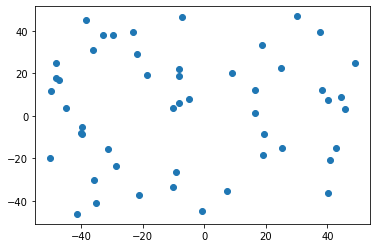
\includegraphics[scale=0.7]{ej1a}
\centering
\end{figure}

\newpage

\textbf{Solución. b)}

\begin{figure}[h]
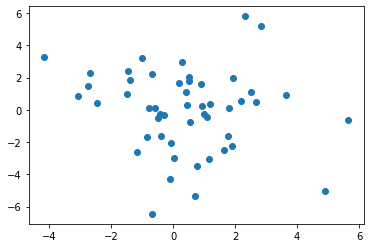
\includegraphics[scale=0.7]{ej1b}
\centering
\end{figure}

\subsection{Valoración de la influencia del rudio en la selección de la complejidad de la clase de funciones.}

\textbf{Enunciado.} Vamos a valorar la influencia del rudio en la selección de la complejidad de la clase de
funciones. Con ayuda de la función simula$\_$unif(100, 2, [50, 50]) generar una muestra de puntos 2D a los que vamos añadir una etiqueta usando el signo de la función $f(x, y) =
y - ax - b$, es decir el signo de la distancia de cada punto a la recta simulada con simula$\_$recta().
\begin{itemize}

\item[a)] Dibujar una gráfica donde los puntos muestren el resultado de su etiqueta, junto con la recta usada para ello. (Observe que todos los puntos están bien clasificados respecto de la recta)

\item[b)] Modifique de forma aleatoria un 10$\%$ etiquetas positivas y otro 10$\%$ de negativas y guarde los puntos con sus nuevas etiquetas. Dibuje de nuevo la gráfica
anterior. ( Ahora hay puntos mal clasificados respecto de la recta)

\item[c)] Supongamos ahora que las siguientes funciones definen la frontera de clasificación de los puntos de la muestra en lugar de una recta :
\begin{itemize}
\item[$\bullet$] $f(x, y) = (x - 10)^2 + (y - 20)^2 - 400$
\item[$\bullet$] $f(x, y) = 0.5(x + 10)^2 + (y - 20)^2 - 400$
\item[$\bullet$] $f(x, y) = 0.5(x - 10)^2 + (y + 20)^2 - 400$
\item[$\bullet$] $f(x, y) = y - 20x^2 - 5x + 3$
\end{itemize}

Visualizar el etiquetado generado en 2b junto con cada una de las gráficas de cada una de las funciones. Comparar las regiones positivas y negativas de estas nuevas funciones
con las obtenidas en el caso de la recta. ¿Son estas funciones más complejas mejores clasificadores que la función lineal? Observe las gráficas y diga que consecuencias extrae sobre la influencia del proceso de modificación de etiquetas en el proceso de
aprendizaje Explicar el razonamiento.

\end{itemize}

\textbf{Solución. a)} Aquí muestro la gráfica con los puntos etiquetados y la recta $y=0.677158x+18.890228$.

\begin{figure}[h]
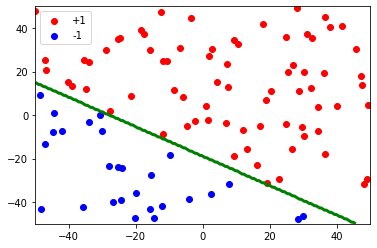
\includegraphics[scale=0.7]{ej2a}
\centering
\end{figure}

Se observa a simple vista que todos los puntos están bien clasificados conforme a la recta.\\

\textbf{Solución. b)} Ahora muestro el gráfico con el ruido indicado. 

\begin{figure}[h]
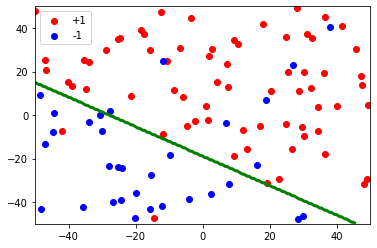
\includegraphics[scale=0.7]{ej2b}
\centering
\end{figure}

Una vez incorporado el ruido indicado, he realizado una medición del error de estas etiquetas conforme a la recta para el siguiente apartado. El error se basa en ver cuantas etiquetas erróneas en porcentaje hay. El 2.94117$\%$ de error en las etiquetas positivas y el 21.875$\%$  en las etiquetas negativas.

\newpage

\textbf{Solución. c)}

\begin{itemize}

\item $f(x, y) = (x - 10)^2 + (y - 20)^2 - 400$

\begin{figure}[h]
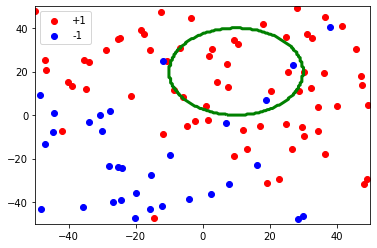
\includegraphics[scale=0.7]{ej2c1}
\centering
\end{figure}

El error que he definido antes, en este caso es el 17.64$\%$ de error en las etiquetas positivas y el 93.75$\%$ de error en las etiquetas negativas.

\item $f(x, y) = 0.5(x + 10)^2 + (y - 20)^2 - 400$

\begin{figure}[h]
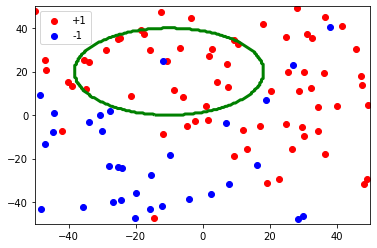
\includegraphics[scale=0.7]{ej2c2}
\centering
\end{figure}

En este caso es el 30.882$\%$ de error en las etiquetas positivas y el 96.875$\%$ de error en las etiquetas negativas. 

\newpage

\item $f(x, y) = 0.5(x - 10)^2 + (y + 20)^2 - 400$

\begin{figure}[h]
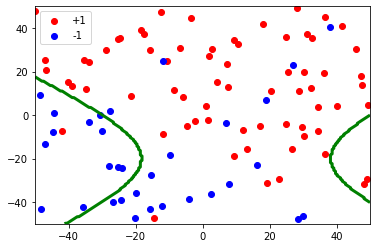
\includegraphics[scale=0.7]{ej2c3}
\centering
\end{figure}

En este caso es el 95.588$\%$ de error en las etiquetas positivas y el 37.5$\%$ de error en las etiquetas negativas.

\item $f(x, y) = y - 20x^2 - 5x + 3$

\begin{figure}[h]
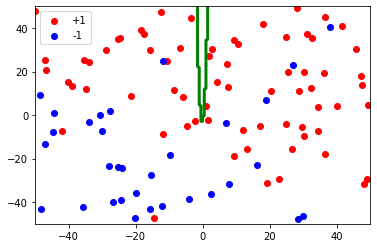
\includegraphics[scale=0.7]{ej2c4}
\centering
\end{figure}

En este caso es el 100.0$\%$ de error en las etiquetas positivas y el 0.0$\%$ de error en las etiquetas negativas.

\end{itemize}

Como podemos ver todos los casos son mucho peores que usando la recta. Esto es debido a que estamos comparando la recta con la que hemos etiquetado con otras funciones, que no tienen ninguna relación.\\

Podemos sacar como conclusión que usar clases de funciones más complejas no implica una mejora en el error. 

\section{Modelos Lineales}

\subsection{Algoritmo Perceptron}

\textbf{Enunciado.} Implementar la función ajusta$\_$PLA(datos, label, max$\_$iter, vini) que calcula el hiperplano solución a un problema de clasificación binaria usando el algoritmo PLA. La entrada datos es una matriz donde cada item con su etiqueta está representado por una fila de la matriz, label el vector de etiquetas (cada etiqueta es un valor +1 o -1), max$\_$iter es el número máximo de iteraciones permitidas y vini el valor inicial del vector. La función devuelve los coeficientes del hiperplano.

\begin{itemize}

\item[1)] Ejecutar el algoritmo PLA con los datos simulados en los apartados 2a de la sección.1. Inicializar el algoritmo con: a) el vector cero y, b) con vectores de
números aleatorios en [0, 1] (10 veces). Anotar el número medio de iteraciones necesarias en ambos para converger. Valorar el resultado relacionando el punto de inicio con el número de iteraciones.

\item[2)] Hacer lo mismo que antes usando ahora los datos del apartado 2b de la sección.1. ¿Observa algún comportamiento diferente? En caso afirmativo diga cual y las
razones para que ello ocurra.

\end{itemize}

\textbf{Solución. 1.a)} En este apartado hemos aplicado el algoritmo PLA sobre nuestra nube de puntos etiquetada sin ruido e inicializando el algoritmo con el vector de pesos (0,0,0). El gráfico resultante es el siguiente: 

\begin{figure}[h]
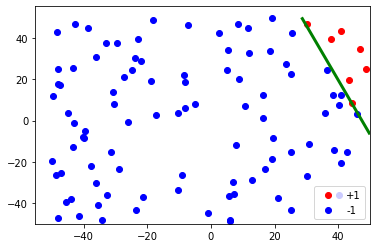
\includegraphics[scale=0.7]{ej2a1a}
\centering
\end{figure}

Este algoritmo, para esta nube de puntos, debe converger ya que no hay ruido y el algoritmo no para hasta que todos los puntos estén bien clasificados. En el caso de arriba la solución a convergido en 444 iteraciones. Obviamente, por lo explicado anteriormente y ante la repetición del algoritmo bajo las mismas condiciones, la media de iteraciones tras 10 ejecuciones es de 444 también.\\

\textbf{Solución. 1.b)} En este apartado hemos aplicado el algoritmo PLA sobre nuestra nube de puntos etiquetada sin ruido e inicializando el algoritmo con el vector de pesos de forma aleatoria entre 0 y 1.\\

Tras ejecutar el algoritmo 10 veces con vectores aleatorios he obtenido una media de 818.1 iteraciones, con iteraciones muy dispares entre puntos. Por eso no podemos sacar ninguna conclusión sobre que haya que empezar en ciertos puntos.\\

\textbf{Solución. 2)} Al añadir ruido a nuestra nube de puntos, por lo explicado en el apartado 1.a, el algoritmo no va a converger. Debido a que no encuentra la solución que clasifica a todos los puntos.\\

He hecho una prueba empírica con 1000 iteraciones y efectivamente el algoritmo no converge. Consigue este resultado:

\begin{figure}[h]
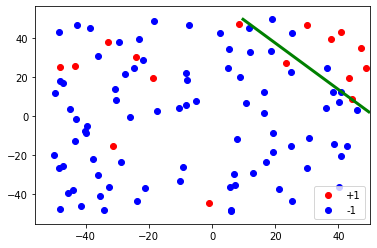
\includegraphics[scale=0.7]{ej2a2}
\centering
\end{figure}

\subsection{Regresión Logística}


\textbf{Enunciado.} En este ejercicio crearemos nuestra propia función objetivo f (una probabilidad en este caso) y nuestro conjunto de datos D para ver cómo funciona regresión logística. Supondremos por simplicidad que f es una probabilidad con valores 0/1 y por tanto que la etiqueta y es una función determinista de x.\\

Consideremos d = 2 para que los datos sean visualizables, y sea $\chi = [0, 2] \times [0, 2]$ con probabilidad uniforme de elegir cada $x \in \chi$. Elegir una línea en el plano que pase por $\chi$ como la frontera entre f(x) = 1 (donde y toma valores +1) y f(x) = 0 (donde y toma valores -1), para ello seleccionar dos puntos aleatorios del plano y calcular
la línea que pasa por ambos. Seleccionar N = 100 puntos aleatorios ${x}_n$ de $\chi$ y evaluar las respuestas ${y}_n$ de todos ellos respecto de la frontera elegida.

\begin{itemize}

\item[1)]Implementar Regresión Logística(RL) con Gradiente Descendente Estocástico (SGD) bajo las siguientes condiciones:

\begin{itemize}

\item[$\bullet$] Inicializar el vector de pesos con valores 0.

\item[$\bullet$]Parar el algoritmo cuando $\Vert w^{(t-1)} - w^{(t)} \Vert < 0.01$, donde $w^{(t)}$ denota el vector de pesos al final de la época t. Una época es un pase completo a través de los N datos.

\item[$\bullet$] Aplicar una permutación aleatoria, 1,2,...,N , en el orden de los datos antes de usarlos en cada época del algoritmo.

\item[$\bullet$] Usar una tasa de aprendizaje de $\eta$ = 0,01

\end{itemize}

\item[2)] Usar la muestra de datos etiquetada para encontrar nuestra solución g y estimar $E_{out}$ usando para ello un número suficientemente grande de nuevas muestras ($>$999).

\end{itemize}

\textbf{Solución. 1)} He implementado el algoritmo de regresión logística con Gradiente descendiente en el cual el tamaño del minibatch es 1.\\

\textbf{Solución. 2)} En el siguiente gráfico muestro la nube de puntos que pide el enunciado con la recta generada al aplicar el algoritmo de regresión logística.\\ 

El número de iteraciones es:  408\\
Los pesos son:  [ 4.0906168 , -8.85518723 , 4.6691689 ]

\begin{figure}[h]
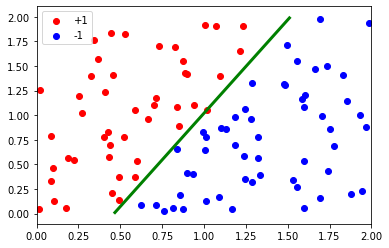
\includegraphics[scale=0.7]{ej2b2}
\centering
\end{figure}

Por último he calculado el $E_{out}$ respectivo a una muestra de test de 1000 puntos y he calculado la media en 1000 poblaciones de 100 puntos:\\

El error generando 1000 poblaciones de 100 puntos uniformes:\\ 
$E_{out}$ medio:  0.09404538317948152\\
El error generando 1000 puntos uniformes:\\
$E_{out}$:  0.09376146145715658\\

Como podemos apreciar el error fuera de la muestra que obtenemos es muy bueno, por lo que hemos conseguido abstraer bastante bien.

\section{Bonus}

\subsection{Clasificación de dígitos}

\textbf{Enunciado.} Considerar el conjunto de datos de los dígitos manuscritos y seleccionar las muestras de los dígitos 4 y 8. Usar los ficheros de entrenamiento
(training) y test que se proporcionan. Extraer las características de intensidad promedio y simetría en la manera que se indicó en el ejercicio 3 del trabajo 1.

\begin{itemize}
\item[a)] Plantear un problema de clasificación binaria que considere el conjunto de entrenamiento como datos de entrada para aprender la función g.
\item[b)] Usar un modelo de Regresión Lineal y aplicar PLA-Pocket como mejora. Responder a las siguientes cuestiones.

\begin{itemize}
\item[1)] Generar gráficos separados (en color) de los datos de entrenamiento y test junto con la función estimada.
\item[2)] Calcular $E_{in}$ y $E_{test}$ (error sobre los datos de test).
\item[3)] Obtener cotas sobre el verdadero valor de $E_{out}$. Pueden calcularse dos cotas una
basada en $E_{in}$ y otra basada en $E_{test}$. Usar una tolerancia $\delta$ = 0.05. ¿Qué cota es mejor?
\end{itemize}

\end{itemize}


\textbf{Solución.}

Para este ejercicio he cogido los datos proporcionados en la práctica dos sobre los dígitos. He seleccionado los datos referentes a los dígitos 4 y 8, para los cuales tenemos las características de intensidad promedio y simetría . Para el etiquetado he asignado un -1 si es 4 y un 1 si es 8.\\

A continuación he representado en un gráfico los conjuntos de training y test obtenidos al aplicar lo anterior:

\newpage

\begin{figure}[h]
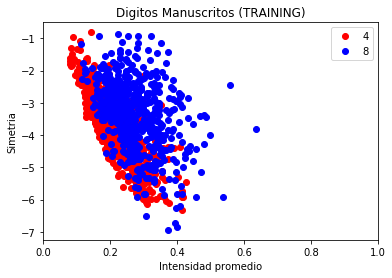
\includegraphics[scale=0.7]{ej3a1}
\centering
\end{figure}

\begin{figure}[h]
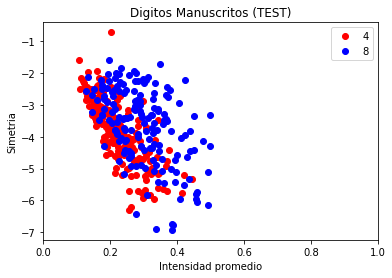
\includegraphics[scale=0.7]{ej3a2}
\centering
\end{figure}

Como modelo de Regresión lineal, he aplicado el \textbf{Gradiente Descendiente Estocástico}, debido a su versatilidad. Y como función de pérdida para este algoritmo he usado:
\begin{align*}
\frac{1}{N} \displaystyle\sum_{n=1}^{N}( w^T x_n - y_n )^2 
\end{align*}

Los resultados obtenidos son malos. El error obtenido en la muestra de training ($E_{in}$) es 0.9273158596798773 y el error en la muestra de test ($E_{test}$) es de 0.9594496935252106

\newpage

\begin{figure}[h]
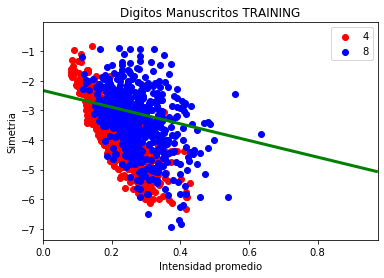
\includegraphics[scale=0.7]{ej3bSGD1}
\centering
\end{figure}

\begin{figure}[h]
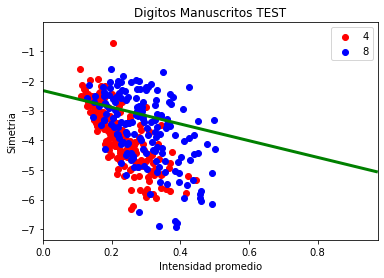
\includegraphics[scale=0.7]{ej3bSGD2}
\centering
\end{figure}

Para mejorar estos resultados vamos a usar el algoritmo \textbf{Pocket}. Es una mejora del perceptron, ya que el gran fallo del perceptron es que siempre cambiamos la solución aunque esta sea peor. Debido a esto, lo que hacemos en el algoritmo pocket es usar el perceptron pero guardando el mejor peso encontrado. Para ello voy a inicializar el algoritmo Pocket con el peso ya encontrado por gradiente descendiente. Para el algoritmo pocket uso la siguiente función de pérdida:
\begin{align*}
\frac{1}{N} \displaystyle\sum_{n=1}^{N}( sign(w^T x_n) \neq y_n ) 
\end{align*}

Al contrario que antes, los resultados obtenidos usando este algoritmo son bastante buenos, con error bajo en la muestra de training y ligeramente superior en la muestra de test, por lo que consigue generalizar bien.\\

El error obtenido en la muestra de training 0.23283082077051925 ($E_{in}$) es  y el error en la muestra de test ($E_{test}$) es de 0.24863387978142076

\begin{figure}[h]
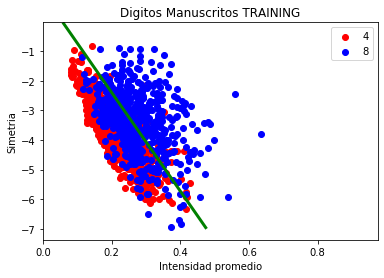
\includegraphics[scale=0.7]{ej3bP1}
\centering
\end{figure}

\begin{figure}[h]
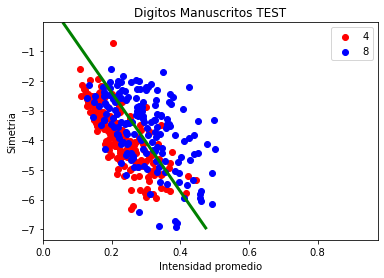
\includegraphics[scale=0.7]{ej3bP2}
\centering
\end{figure}

Por último vamos a sacar una cota para el error en la población ($E_{out}$). Para ello voy a usar la desigualdad de Hoeffding:
\begin{align*}
P(D:\|E_{out}(g)-E_{in}(g)\|>\varepsilon)\leq 2e^{-2\varepsilon^2N}, \forall \varepsilon >0
\end{align*}

\newpage

De la cual, operando y considerando $\delta = 2e^{-2\varepsilon^2N}$, obtenemos con probabilidad $ 1 - \delta $ sobre D: 
\begin{align*}
E_{out}(g) \leq E_{in}(g) + \sqrt{\frac{1}{2N}log(\frac{2}{\delta})} 
\end{align*}

Por tanto, puedo calcular las cotas. Las cotas calculadas son al 95$\%$ de probabilidad.\\

Usando $E_{in}$ : $E_{out} \leq  0.2884142155990554$\\
Usando $E_{test}$ : $E_{out} \leq  0.349027632636532$


\end{document}
